\section{Cr�er une image}
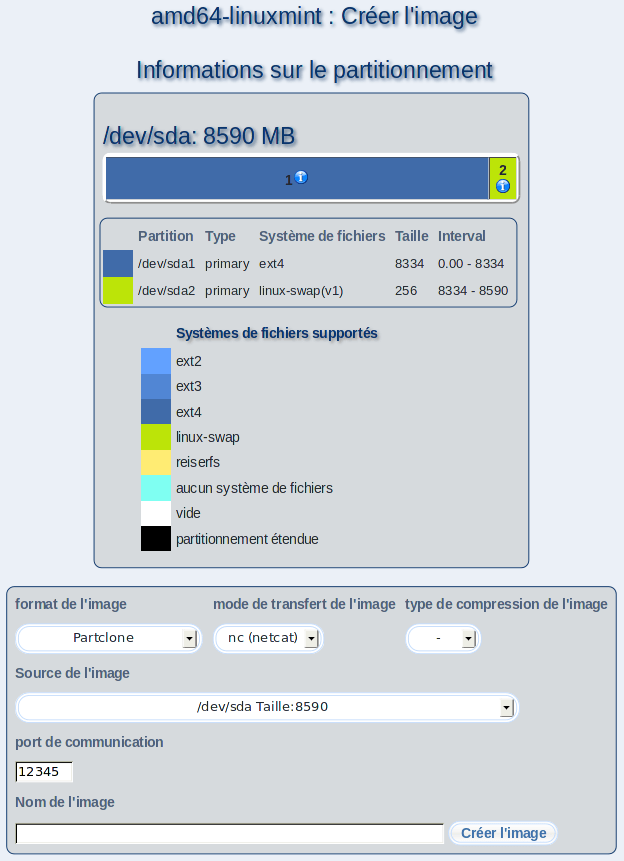
\includegraphics[scale=0.4]{/mdk/doc/manual/screenshots/fr/client_createImage.png} \\
En utilisant ce dialogue, vous pouvez cr\'eer des fichiers image des partitions ou des lecteurs entiers d'un poste client que vous pouvez utiliser pour l'installation des postes client ult\'erieurs. Pour cela, choisissez le format d'image souhait\'e, le mode de transfert de l'image et la compression de l'image. D\'ependant du format de l'image, il est n\'ecessaire que vous entrez des informations additionelles chez \textit{�Source de l'image�}, par exemple quelle partition ou quel lecteur doit \^etre enregistr\'ee dans le fichier image.\\
Puis, choisissez un nom pour votre fichier et entrez-le chez \textit{�Nom de l'image�}. Enfin, cliquez sur \textit{�Cr�er une image�}.\\
\subsection{Les fichiers image}
Les fichiers seront enregistr\'es dans le r\'epertoire \textbf{/m23/data+scripts/clientImages}. Il peuvent \^etre comprim\'es avec des formats diff\'erents et avec des m\'ethodes diff\'erentes. Le sch\'ema de leur nom, quand m\^eme, est toujours le m\^eme: $\langle$nom de l'image$\rangle$$\langle$taille de l'image decomprim\'ee en bytes$\rangle$$\langle$format de l'image$\rangle$$\langle$compression$\rangle$\\
Le format de l'image peut \^etre comme ceci:\\
\begin{itemize}
\item \textbf{dd}: Toutes les donn\'ees d'une partition ou d'un lecteur seront enregistr\'ees.\\
\end{itemize}
Pour la compression, les valeurs suivantes sont valides:\\
\begin{itemize}
\item  (aucune extension de compression): Le fichier image n'est pas comprim\'e.\\
\item \textbf{gz}: La compression sera ex\'ecut\'ee avec le programme gzip.\\
\item \textbf{bz2}: La compression sera ex\'ecut\'ee avec le programme bzip2 (ce qui est plus fort dans la plupart des cas).\\
\end{itemize}
\subsection{La connexion de transfert}
Pour le mode de transfert de l'image, il est n\'ecessaire que vous indiquiez une connexion de r\'eseau qui peut \^etre utilis\'ee de la cot\'e du poste client et du serveur et qui n'est pas bloqu\'ee par un pare-feu etc. Si vous voudriez cr\'eer des plusieures images au m\^eme temps, vous devez choisir des connexions diff\'erentes.\\
